The basic idea of our framework is to construct a surrogate model using the theory of polynomial chaos (PC) expansions. Given such a surrogate model, quantities as cumulative distributions functions (\cdfs) and \pdfs\ can be trivially estimated. Moreover, the representations, which we compute, provide analytical formulae for probabilistic moments, \ie, the expected value, variance, \etc\ are readily available.

\subsection{Outline of the Framework}
The major steps of our technique are depicted in \fref{algorithm}:

\stage{1}{Uncertain Parameters (\sref{uncertain-parameters}).} The PC expansions operate on mutually independent \rvs. The uncertain parameters $\vU(\o)$ might not satisfy this requirement and, therefore, should be preprocessed; we shall denote the corresponding independent set of \rvs\ by $\vZ(\o)$.

\stage{2}{Power Model (\sref{power-model}).} The user specifies the power model of the system via a ``black-box'' functional $\f$, which outputs the total power $\vP(\t, \o)$ for a particular temperature $\vTO(\t, \o)$ and an outcome of the parameters $\vU(\o)$.

\stage{3}{Thermal Model (\sref{thermal-model}).} With respect to the thermal specification $\system$ defined in \sref{problem-formulation}, a mathematical model of the thermal system is constructed. The thermal model closely interacts with the power model from \stage{2}\ and produces the corresponding temperature profile.

\stage{4}{Surrogate Model (\sref{polynomial-chaos}).} The surrogate model is attained by traversing the desired time span and gradually constructing polynomial expansions, in terms of the processed uncertain parameters $\vZ(\o)$ from \stage{1}, for the stochastic power and temperature profiles. The output is essentially a substitute for the model produced at \stage{3}\ with respect to the power model determined at \stage{2}.

\stage{5}{Post-processing (\sref{output-processing}).} The computed PC expansions are analyzed in order to obtain the desired characteristics of the system, \eg, \cdfs, \pdfs, moments.


\subsection{Application to Process Variation} \slabel{overview-application}
Before diving into details, we show a particular application of the proposed framework. Specifically, we shall perform stochastic PTA of a dual-core platform, wherein the parameters that affect the leakage current are uncertain. The application is a simplified version of the example in \sref{illustrative-example}; hence, all the omitted details will be described later on.

\begin{figure}[t]
  \vspace{-1.0em}
  \centering
  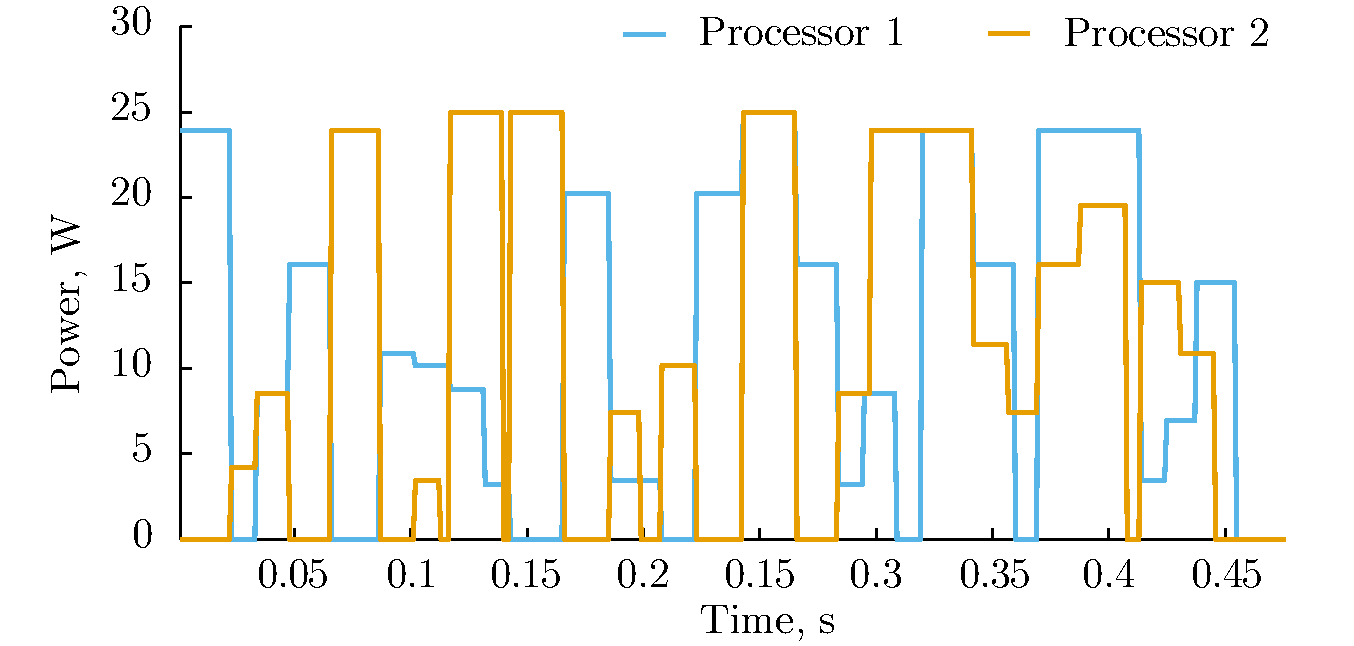
\includegraphics[width=0.90\columnwidth]{include/assets/application-power.pdf}
  \caption{A dynamic power profile.}
  \flabel{power}
  \vspace{-1.5em}
\end{figure}

\begin{figure}
  \centering
  \updatedFigure{
  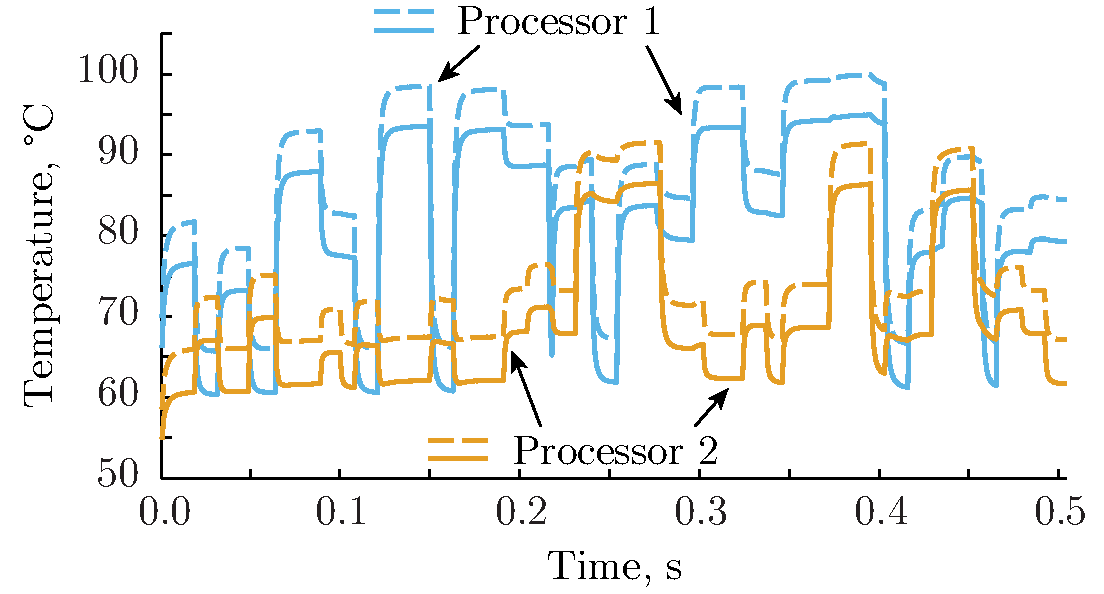
\includegraphics[width=0.90\columnwidth]{include/assets/application-temperature.pdf}
  }
  \vspace{-1.0em}
  \caption{The expected temperature (the solid lines) and one standard deviation above it (the dashed lines).}
  \flabel{application-temperature}
  \vspace{-1.0em}
\end{figure}

Without loss of generality, we address one of the most critical leakage parameters: the effective channel length \cite{chandra2010, juan2011, juan2012, srivastava2010, shen2009}. Due to process variation, the channel length is a \rv, which we denote by $\Leff(\o)$. The variations of $\Leff(\o)$ are split into global (inter-die) $\gLeff(\o)$ and local (intra-die) $\lLeff(\o)$ parts. Assume $\gLeff(\o)$ is shared among the two processors whereas each processor has its own local \rv\ $\lLeff_i(\o)$. Therefore, the channel length of the $i$th processor is
\begin{equation} \elabel{leakage-partition}
  \Leff_i(\o) = \nLeff + \gLeff(\o) + \lLeff_i(\o)
\end{equation}
where $\nLeff$ is the nominal value. Thus, the uncertain parameters, $\vU(\o)$, of the problem have been identified, \ie,
\[
  \vU(\o) = \vec{\lLeff_1(\o), \; \lLeff_2(\o), \; \gLeff(\o) }.
\]
The variations of $\Leff(\o)$ can be accurately approximated by Gaussian distributions \cite{juan2011, juan2012, srivastava2010}; hence, we assume that $\vU(\o)$ is a Gaussian vector with a given covariance matrix. Since the local \rvs\ are known to have spacial correlations, the uncertain parameters $\vU(\o)$ are not independent. Therefore, at \stage{1}\ of our framework, we transform $\vU(\o)$ into a set of independent \rvs\ denoted by $\vZ(\o) = \vec{\Z_1(\o), \; \Z_2(\o)}$, which is also Gaussian. Note, due to the correlations among $\lLeff_i(\o)$, we were also able to reduce the number of \rvs\ to two making the modeling more efficient. At \stage{2}, we decide on the power model; assume it is given as the following closed-form formula (denoted by $\f$ in \fref{algorithm}):
\begin{align*}
  & \P_i(\t, \o) = \P_{\dyn, i}(\t) + \beta_i \: \exp \left(\vphantom{\T^2_i} \alpha_0 + \alpha_1 \: \Leff_i(\o) \right. \\
  & \qquad {} + \left. \alpha_2 \: \T_i(\t, \o) + \alpha_3 \: \Leff_i(\o) \: \T_i(\t, \o) + \alpha_4 \: \T_i(\o, \t)^2 \right),
\end{align*}
for $i = 1, 2$, where $\P_{\dyn, i}(\t)$ is the dynamic power, and the rest belongs to the leakage power, which is a measurement-based model of the corresponding electrical circuits with the fitting coefficients $\alpha_j$ and $\beta_i$. Due to the separation of the dynamic and leakage parts, we only need to perform one system/power simulation of the system under the desired workload \emph{without} considering leakage and dump the corresponding nominal dynamic power profile, $\profPdyn$, of this workload; the leakage part will be added afterwards. Assume the resulting $\profPdyn$ is the one shown in \fref{application-power}. We move on to the thermal model, \stage{3}. The thermal specification $\system$ of the system at hand is assumed to be given; in particular, the floorplan of the die and the configuration of the thermal package are known. Therefore, we construct an equivalent RC thermal circuit of the system, which is depicted in \fref{circuit} in the appendix. Hence, a mathematical model of heat transfer within the platform is acquired. We transform this model in a certain way and denote the result by $\mCF(\t)$ and $\mCS(\t)$ in \fref{algorithm}. At \stage{4}, the independent \rvs, power model, and thermal model are fused together under the desired workload to produce the corresponding stochastic power $\profP{\o}$ and temperature $\profT{\o}$ profiles. The obtained stochastic profiles are nothing more than two polynomials of $\Z_1(\o)$ and $\Z_2(\o)$ with time-dependent coefficients. For example, assuming a second-total-order PC expansion, the temperature at the $k$th moment of times is
\begin{align*}
  \vTO_k(\o) &= \pccs_{k1} + \pccs_{k2} \Z_1(\o) + \pccs_{k3} \Z_2(\o) + \pccs_{k4} \Z_1(\o) \Z_2(\o) \\
  & \qquad \qquad {} + \pccs_{k5} (\Z_1(\o)^2 - 1) + \pccs_{k6} (\Z_2(\o)^2 - 1)
\end{align*}
where $\pccs_{ki}$ are vectors with two elements corresponding to the two processors. The expansion for power has the same structure but different coefficients. Such a series might be shorter or longer depending on the accuracy requirements. As we see, our surrogate model has a negligibly small computational cost to undertake UQ at \stage{5}: for any outcome of the uncertain parameters $\vZ(\o) \equiv \vZ$, we can easily compute the corresponding temperature by plugging $\vZ$ into the above equation; the same applies for power. Furthermore, the expectation and variance are calculated as simply as
\[
  \oExp{\vTO_k(\o)} = \pccs_{k1} \hspace{1em} \text{and} \hspace{1em} \oVar{\vTO_k(\o)} = \sum_{i = 2}^{6} \pcn_i \: \pccs_{ki}^2
\]
where $\pcn_i$ are normalization constants, and the squaring should be understood element-wise. For the nominal power profile $\profPdyn$ depicted in \fref{application-power}, we obtain the corresponding stochastic temperature profile $\profT{\o}$ and can observe, \eg, its expectation and standard deviation; they are plotted in \fref{application-temperature}. The displayed curves closely match those obtained via MC simulations with $10^4$ samples; however, our method takes less than a second, on a personal laptop, while the MC-based approach takes more than a day, which we shall discuss in \sref{experimental-results}. Finally, it is worth being noted that \stage{1}--\stage{2}\ are fixed for a particular platform, \ie, the corresponding outputs are tabulated and have no additional costs. In other words, various workloads of the system can be efficiently analyzed by constructing PC expansions at \stage{4}\ followed by the post-processing at \stage{5}.

